\section{Cálculos de poder}
Este experimento cuenta con estrictamente con 36 tratamientos si la combinación de cada vestimenta, con cada habilidad y cada aspiración es considerada un tratamiento. Si en cambio las vestimentas son agrupadas en tres categorías (femenina, masculina y ambigua/neutral), el experimento tiene 8 tratamientos. Los siguientes cálculos de poder supone son 8 tratamientos. 

Para detectar un efecto de 0.15d,e con un nivel de significancia de 0.05, con un poder del 80\% es necesario tener una muestra de $1,396$ por tratamiento (ver Figura \ref{fig:calc} ). Es decir, en total era necesario tener una muestra de $11,168$ para tener 80\% de poder para ver efectos de 0.15d.e. Para ver efectos de 0.3d.e con una significancia de 0.05 y un poder del 80\% era necesario tener en total un muestra de $2,792$ (ver Figura \ref{fig:calc}). Ahora, con la muestra de este trabajo el poder para detectar efectos de 0.15d.e es del 10\% y para detectar efectos de 0.3d.e es de 25\%.

\begin{figure}[!ht]
    \centering
    \caption{Cálculos de poder}
    \begin{subfigure}{\textwidth}
        \centering
        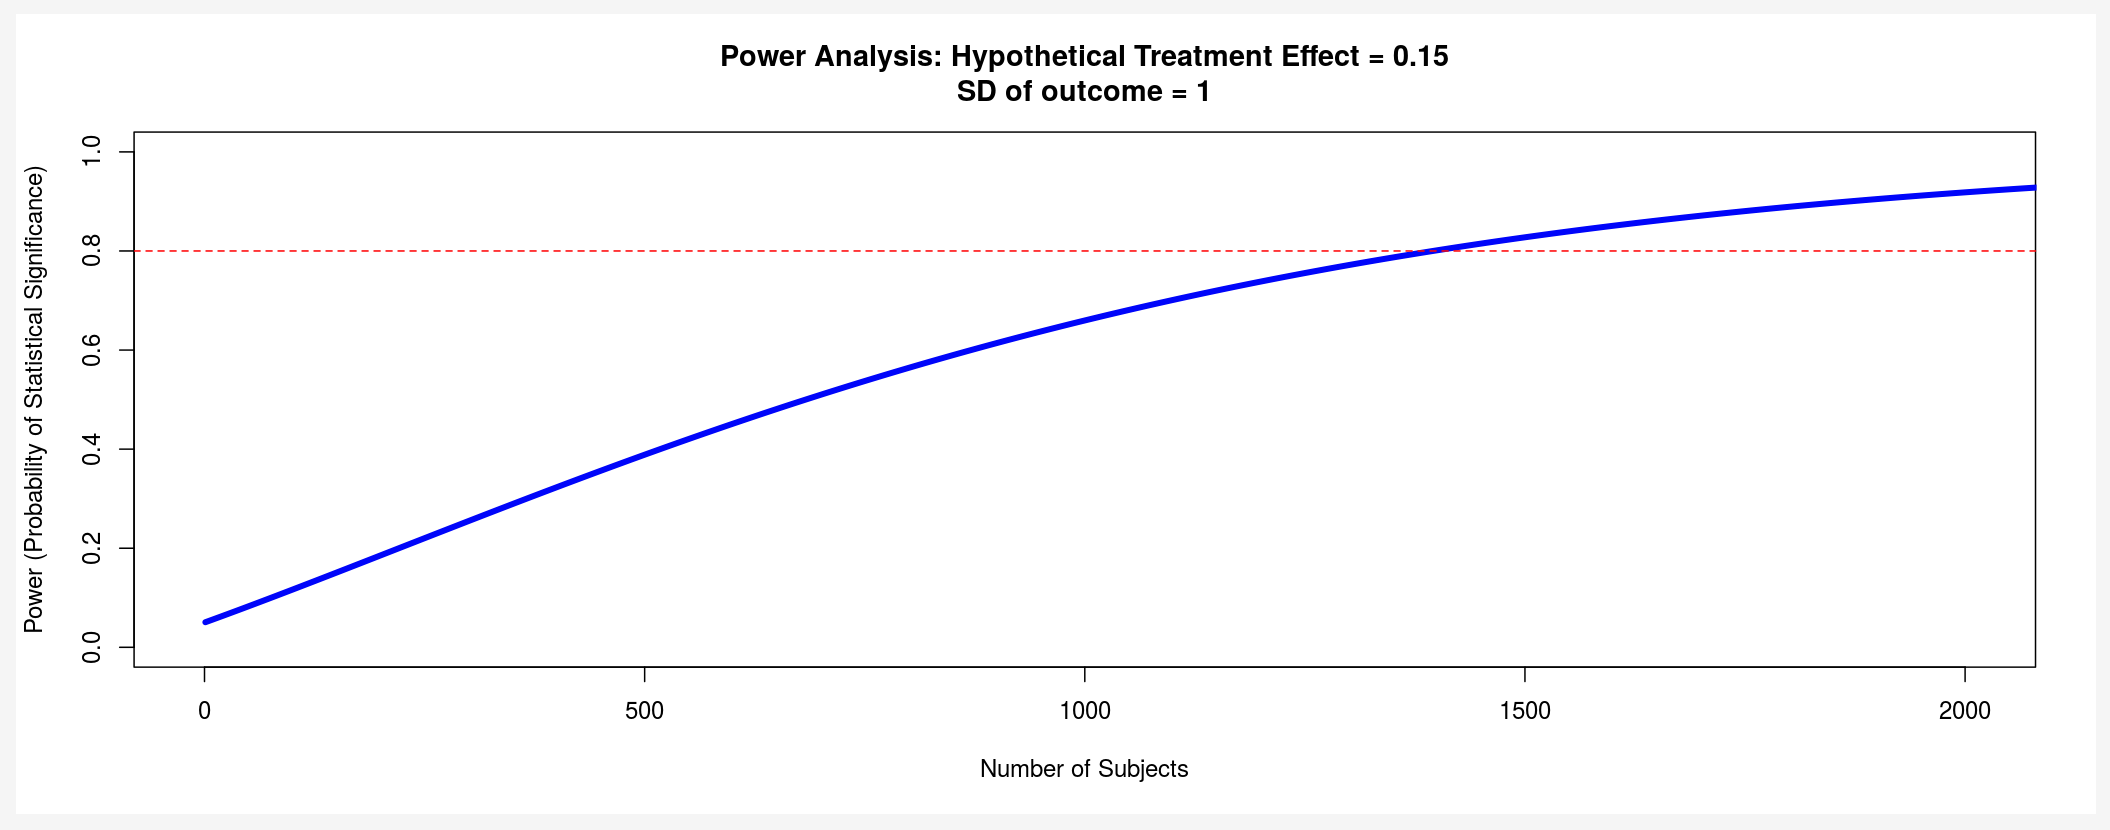
\includegraphics[width=13cm]{Images/pc_15.png}
        %\caption{Muestra necesaria para observar efectos de 0.15d.e con 80\% de poder}
    \end{subfigure}
    \begin{subfigure}{\textwidth} 
        \centering
        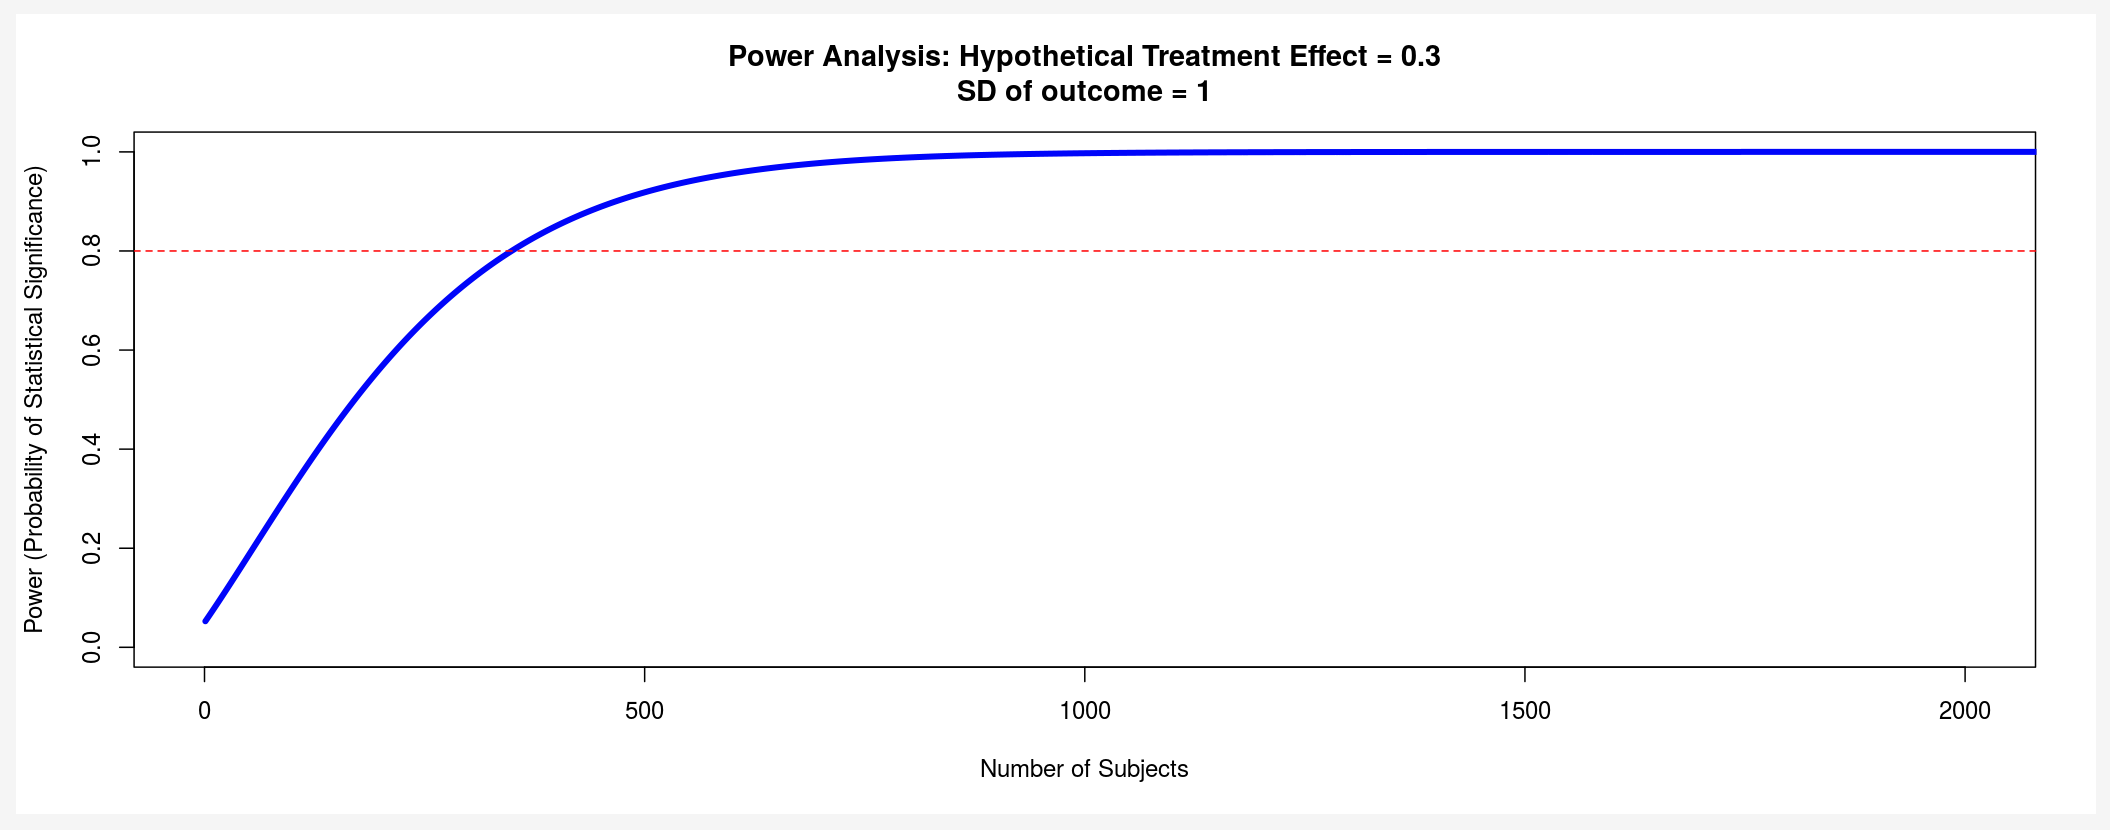
\includegraphics[width=13cm]{Images/pc_30.png}
        %\caption{Muestra necesaria para observar efectos de 0.3d.e con 80\% de poder}
    \end{subfigure}
    \label{fig:calc}
    \begin{singlespace}
        \floatfoot{\footnotesize{\textbf{Fuente:} Egap Power Tool }\par}
    \end{singlespace}
\end{figure}
